% Options for packages loaded elsewhere
\PassOptionsToPackage{unicode}{hyperref}
\PassOptionsToPackage{hyphens}{url}
\PassOptionsToPackage{dvipsnames,svgnames,x11names}{xcolor}
%
\documentclass[
  11pt,
  letterpaper,
]{article}
\usepackage{amsmath,amssymb}
\usepackage{lmodern}
\usepackage{iftex}
\ifPDFTeX
  \usepackage[T1]{fontenc}
  \usepackage[utf8]{inputenc}
  \usepackage{textcomp} % provide euro and other symbols
\else % if luatex or xetex
  \usepackage{unicode-math}
  \defaultfontfeatures{Scale=MatchLowercase}
  \defaultfontfeatures[\rmfamily]{Ligatures=TeX,Scale=1}
\fi
% Use upquote if available, for straight quotes in verbatim environments
\IfFileExists{upquote.sty}{\usepackage{upquote}}{}
\IfFileExists{microtype.sty}{% use microtype if available
  \usepackage[]{microtype}
  \UseMicrotypeSet[protrusion]{basicmath} % disable protrusion for tt fonts
}{}
\makeatletter
\@ifundefined{KOMAClassName}{% if non-KOMA class
  \IfFileExists{parskip.sty}{%
    \usepackage{parskip}
  }{% else
    \setlength{\parindent}{0pt}
    \setlength{\parskip}{6pt plus 2pt minus 1pt}}
}{% if KOMA class
  \KOMAoptions{parskip=half}}
\makeatother
\usepackage{xcolor}
\IfFileExists{xurl.sty}{\usepackage{xurl}}{} % add URL line breaks if available
\IfFileExists{bookmark.sty}{\usepackage{bookmark}}{\usepackage{hyperref}}
\hypersetup{
  pdftitle={Modeling age patterns of childlessness: a semi-parametric approach},
  colorlinks=true,
  linkcolor={blue},
  filecolor={Maroon},
  citecolor={blue},
  urlcolor={blue},
  pdfcreator={LaTeX via pandoc}}
\urlstyle{same} % disable monospaced font for URLs
\usepackage[margin=25mm]{geometry}
\usepackage{longtable,booktabs,array}
\usepackage{calc} % for calculating minipage widths
% Correct order of tables after \paragraph or \subparagraph
\usepackage{etoolbox}
\makeatletter
\patchcmd\longtable{\par}{\if@noskipsec\mbox{}\fi\par}{}{}
\makeatother
% Allow footnotes in longtable head/foot
\usepackage{footnote} % For some unknown reason, footnotehyper clashes with French
\makesavenoteenv{longtable}
\usepackage{graphicx}
\makeatletter
\def\maxwidth{\ifdim\Gin@nat@width>\linewidth\linewidth\else\Gin@nat@width\fi}
\def\maxheight{\ifdim\Gin@nat@height>\textheight\textheight\else\Gin@nat@height\fi}
\makeatother
% Scale images if necessary, so that they will not overflow the page
% margins by default, and it is still possible to overwrite the defaults
% using explicit options in \includegraphics[width, height, ...]{}
\setkeys{Gin}{width=\maxwidth,height=\maxheight,keepaspectratio}
% Set default figure placement to htbp
\makeatletter
\def\fps@figure{htbp}
\makeatother
\setlength{\emergencystretch}{3em} % prevent overfull lines
\providecommand{\tightlist}{%
  \setlength{\itemsep}{0pt}\setlength{\parskip}{0pt}}
\setcounter{secnumdepth}{5}
\newlength{\cslhangindent}
\setlength{\cslhangindent}{1.5em}
\newlength{\csllabelwidth}
\setlength{\csllabelwidth}{3em}
\newlength{\cslentryspacingunit} % times entry-spacing
\setlength{\cslentryspacingunit}{\parskip}
\newenvironment{CSLReferences}[2] % #1 hanging-ident, #2 entry spacing
 {% dont indent paragraphs
  \setlength{\parindent}{0pt}
  % turn on hanging indent if param 1 is 1
  \ifodd #1
  \let\oldpar\par
  \def\par{\hangindent=\cslhangindent\oldpar}
  \fi
  % set entry spacing
  \setlength{\parskip}{#2\cslentryspacingunit}
 }%
 {}
\usepackage{calc}
\newcommand{\CSLBlock}[1]{#1\hfill\break}
\newcommand{\CSLLeftMargin}[1]{\parbox[t]{\csllabelwidth}{#1}}
\newcommand{\CSLRightInline}[1]{\parbox[t]{\linewidth - \csllabelwidth}{#1}\break}
\newcommand{\CSLIndent}[1]{\hspace{\cslhangindent}#1}

%%%%%%%% START HEADER PARTIAL %%%%%%%%%%%%

% Formatting of tables & knitr::kable and kableExtra functionality
\usepackage{float}
\usepackage{colortbl}
\usepackage{pdflscape}
\usepackage{tabu}
\usepackage{threeparttable}

% Line numbering

% endfloat stuff

% fancyhdr pagestyle

% Environment for keywords
\makeatletter
\newcommand\keywordsname{Keywords}
\newenvironment*{keywords}[1][\keywordsname]{\if@twocolumn \else \small \quotation \fi \begin{center} \textbf{\textit{#1} \\}}{\end{center}\if@twocolumn \else \small \endquotation \fi}
\newenvironment*{keywordsinline}[1][\keywordsname]{\if@twocolumn \else \small \quotation \fi \begin{center} \textbf{\textit{#1}: }}{\end{center}\if@twocolumn \else \small \endquotation \fi}
\makeatother

% Environment for abstract that takes new abstract name
\newenvironment{renameableabstract}[1][\abstractname]{\let\oldabstractname\abstractname \renewcommand{\abstractname}{#1} \begin{abstract}}{\end{abstract} \renewcommand{\abstractname}{\oldabstractname}}

%%%%%%%% END HEADER PARTIAL %%%%%%%%%%%%

\ifLuaTeX
  \usepackage{selnolig}  % disable illegal ligatures
\fi

\title{Modeling age patterns of childlessness: a semi-parametric approach}

%%%%%%% START AUTHOR PARTIAL %%%%%%%%%%%%%%%

%%%%% Authors, affiliations and author notes stuff %%%%%

% Macros for creating and referencing stored reference
\makeatletter
\def\MyNewLabel#1#2#3{\expandafter\gdef\csname #1@#2\endcsname{#3}}

\def\MyRef#1#2{\@ifundefined{#1@#2}{???}{\csname #1@#2\endcsname}}

\newcommand*\ifcounter[1]{%
  \ifcsname c@#1\endcsname
    \expandafter\@firstoftwo
  \else
    \expandafter\@secondoftwo
  \fi
}
\makeatother

% Create labels for Addresses if the are given by code
\MyNewLabel{ADDRTXT}{A}{Department of Statistical Sciences, University of Toronto, Canada}
\MyNewLabel{ADDRTXT}{B}{Departments of Statistical Sciences and Sociology, University of Toronto, Canada}

% Create labels for Footnotes if they are given by code
\MyNewLabel{ANOTETXT}{corresp}{\href{mailto:benjamin.schluter@utoronto.ca}{\nolinkurl{benjamin.schluter@utoronto.ca}}.}

%%% Special footnotes for addresses and author footnotes
\usepackage{bigfoot}
\DeclareNewFootnote{Addr}[arabic] % Only used for NOT authblk
\DeclareNewFootnote{ANote}[fnsymbol]

%%% Address and author notes as a function of format %%%
 % Use authblk for affiliations %%%%%%%%%%%
\usepackage{authblk}

% Always separate by commas
\renewcommand\Authsep{, }
\renewcommand\Authand{, }
\renewcommand\Authands{, }

% Counter for addresses and footnotes
\newcounter{addrcnt}

% thanks definition that doesnt produce superscript marks
\makeatletter
\newcommand*\createaddrlblbycode[1]{%
  \ifcounter{ADDRLBL@#1}
    {}
    {\refstepcounter{addrcnt}\newcounter{ADDRLBL@#1}\setcounter{ADDRLBL@#1}{\value{addrcnt}}}%
}

\newcommand*\addrlblbycode[1]{\arabic{ADDRLBL@#1}}

\newcommand*\addrbycode[1]{%
  \ifcounter{ADDR@#1}
    {}
    {\newcounter{ADDR@#1}%
     \affil[\addrlblbycode{#1}]{\MyRef{ADDRTXT}{#1}}}%
}

\newcommand*\createanotelblbycode[1]{%
  \ifcounter{ANOTELBL@#1}
    {}
    {\refstepcounter{footnoteANote}\newcounter{ANOTELBL@#1}\setcounter{ANOTELBL@#1}{\value{footnoteANote}}}%
}

\newcommand*\anotelblbycode[1]{\fnsymbol{ANOTELBL@#1}}

\newcommand*\anotebycode[1]{%
  \ifcounter{ANOTE@#1}
    {}
    {\newcounter{ANOTE@#1}%
     \footnotetextANote[\value{ANOTELBL@#1}]{\MyRef{ANOTETXT}{#1}}}%
}
\makeatother


\createaddrlblbycode{A}


\createanotelblbycode{corresp}

\author[%
\addrlblbycode{A}%
,%
$\anotelblbycode{corresp}$%
]{Benjamin-Samuel Schluter}

\addrbycode{A}


\createaddrlblbycode{B}



\author[%
\addrlblbycode{B}%
]{Monica Alexander}

\addrbycode{B}


%endif(authblk)

%%%%%%%%% END AUTHOR PARTIAL %%%%%%%%

\date{}

\begin{document}
\maketitle

%%%%%%%%%% START AFTER TITLE PARTIAL %%%%%%%%%%%%%
\anotebycode{corresp}


%%%%%%%%%% END AFTER TITLE PARTIAL %%%%%%%%%%%%%

\begin{abstract}
Trends and patterns in childlessness are important to measure and understand its relationship with fertility rates and fertility intentions. However, data on childlessness is often limited to survey data, which suffers from small sample sizes for key subpopulations. We propose a model estimating age-specific proportions of individuals being childless at a subnational level. The model consists of an `expected' component -- capturing the shape of childlessness over age using a logistic function -- and deviations from the expected level, modeled with P-splines. The model estimates summary parameters which are useful to understand trends over time. The model is estimated in a Bayesian framework allowing temporal smoothing and pooling of the parameters. We apply the model to estimate the proportions of childless women by race/ethnicity in the U.S. The preliminary results are promising and the model could be expanded to model multiple parities and perform projection of childlessness.
\end{abstract}

\hypertarget{introduction}{%
\section{Introduction}\label{introduction}}

Childlessness is a demographic phenomenon that has gained increased attention, particularly in high-income countries characterized by low fertility rates. The share of childless American women aged 40 to 44 was 10\% in 1976, reached a peak at 20\% in 2005, and fall hereafter to 15\% in 2014 (\protect\hyperlink{ref-livingston2015childlessness}{Livingston 2015}). In line with previous results, Dye (\protect\hyperlink{ref-dye2010fertility}{2010}) showed that among American women aged 45 in 2006, one fifth were childless. While prior studies focused on female childlessness, recent years also brought research on male childlessness (\protect\hyperlink{ref-gray2013childbearing}{Gray, Evans, and Reimondos 2013}; \protect\hyperlink{ref-nisen2014age}{Nisén et al. 2014}).

Trends and patterns in childlessness are important to understand, both in terms of the relationship with overall fertility, and whether trends match with trends in fertility intentions. This has motivated research trying to identify its causes, determinants and consequences (\protect\hyperlink{ref-dykstra2007pathways}{Dykstra and Wagner 2007}; \protect\hyperlink{ref-gemmill2019some}{Gemmill 2019}; \protect\hyperlink{ref-kendig2007health}{Kendig et al. 2007}; \protect\hyperlink{ref-kirmeyer2011childbearing}{Kirmeyer and Hamilton 2011}; \protect\hyperlink{ref-mynarska2015diverse}{Mynarska et al. 2015}).

Despite the increasing attention received by childlessness, no modeling framework has been proposed to estimate the age-specific share of individuals not having a child. A statistical model is particularly relevant when
obtaining age-specific childlessness proportions in small subpopulations. Indeed, small population sizes lead to high stochasticity in the raw data, rendering the underlying trend unclear. For example, it has been shown that the proportion of women childless varies across racial/ethnic groups (\protect\hyperlink{ref-livingston2015childlessness}{Livingston 2015}; \protect\hyperlink{ref-lundquist2009race}{Lundquist, Budig, and Curtis 2009}) but not much is known about the patterns of subpopulations defined by different combination of individual characteristics such as the state of residence, race/ethnicity, and education level.

In this paper we propose a model framework to estimate age-specific proportions of individuals being childless at a subnational and subpopulation level. The model is semi-parametric in the sense that we allow some deviations from an expected level parametrized by a logistic function. The logistic function estimates the entire age schedule proportions of childless individuals with three parameters that are smoothed over time. This semi-parametric framework is robust to zero counts while being flexible. We show preliminary results as applied to race--specific childlessness proportion in the U.S. Future work will expand the model to allow estimating population subgroups defined by a combination of factors (i.e.~state of residence and race/ethnicity).

\hypertarget{modeling-framework}{%
\section{Modeling Framework}\label{modeling-framework}}

Define \(y_{x, g, t}\) to be the number of childless persons of age \(x\) belonging to subpopulation group \(g\) at time \(t\). Define \(n_{x, g, t}\) to be the subpopulation group \(g\) aged \(x\) at time \(t\). We assume the counts of parent to be Binomially distributed as follows,

\[y_{x, g, t}|\theta_{x,g,t} \sim \text{Binomial}(n_{x, g, t}, \theta_{x,g,t}).\]
Our aim is to estimate the proportion being childless \(\theta_{x,g,t}\). We model these proportions on the logit scale as follows,

\[\text{logit}(\theta_{x,g,t}) = \text{logit}(1 - f(\zeta_{g, t}, \gamma_{g, t}, \delta_{g, t})) + \sum_k B_{x,k} \alpha_{k,g,t}\]
where

\[f(\zeta_{g, t}, \gamma_{g, t}, \delta_{g, t}) =  \frac{\zeta_{g, t}}{1+e^{-\gamma_{g, t}(x-\delta_{g, t})}}\]

is the logistic function with \(\delta\) the function's midpoint, \(\zeta\) the supremum of the values of the function, and \(\gamma\) the steepness of the curve. Deviations from the parametric function are modeled with P-splines (\protect\hyperlink{ref-eilers1996flexible}{Eilers and Marx 1996}). More precisely, \(\boldsymbol{B}\) is the cubic basis matrix of dimension (\(A \times K\)) where \(A=44\) the upper age bound, and \(K=6\) the number of knots; \(\boldsymbol{\alpha_{g,t}}\) is a cubic-splines parameter vector of dimension (\(K \times 1\)) estimated in the model. We impose smoothness on the deviations by using a Random Walk 1 prior on \(\boldsymbol{\alpha_{g,t}}\),

\[\alpha_{k,g,t} \sim \text{Normal}(\alpha_{k-1,g,t}, \sigma_{\alpha, t}^2)\]
where the variance parameter \(\sigma_{\alpha,t}^2\) is shared across all subpopulation groups in each year.

Following exploratory data analyses, we smooth the logistic parameters by assuming that

\[\zeta_{g,t} \sim \text{Normal}(\zeta_{g,t-1}, \sigma_{\zeta}^2)\]
\[\gamma_{g,t} \sim \text{Normal}(\gamma_{g,t-1}, \sigma_{\gamma}^2)\]
and

\[\delta_{g,t} \sim \text{Normal}(2\cdot \delta_{g,t-1} - \delta_{g,t-2}, \sigma_{\delta}^2).\]
The variance parameters are shared across all subpopulation groups to enforce some pooling of information. All variance parameters take \(\text{Normal}(0,1)^+\) priors (weakly informative priors).

Our set-up resembles the TOPALS (\protect\hyperlink{ref-de2012smoothing}{De Beer 2012}; \protect\hyperlink{ref-gonzaga2016estimating}{Gonzaga and Schmertmann 2016}) and P-TOPALS (\protect\hyperlink{ref-dyrting2020smoothing}{Dyrting 2020}) models except that in our case, the expected level is estimated.

\hypertarget{preliminary-results}{%
\section{Preliminary Results}\label{preliminary-results}}

\hypertarget{data}{%
\subsection{Data}\label{data}}

We test our model on the proportion being childless by race/ethnicity using Current Population Surveys (CPS) data Fertility and Marriage June supplement. The survey has been conducted every two years\footnote{Except for the year 1996 which was collected in 1995 instead.} and we consider the period 1990-2020. We define childlessness with the variable ``frever'' which indicates the number of live birth a women ever had. A women of a given age was defined childless when ``frever'' was equal to zero. Women considered are aged 15 to 44 years old. The variables ``race'' and ``hispan'' were combined to construct the racial/ethnic categories: ``non-Hispanic Black'', ``non-Hispanic White'', and ``Hispanic''. The obtained counts were adjsuted based on survey weights.

\hypertarget{preliminary-results-1}{%
\subsection{Preliminary results}\label{preliminary-results-1}}

Figure \ref{fig:race-fit} shows the percent of women childless (y-axis) over the ages 15 to 44 years old (x-axis) for the three racial/ethnic groups considered (horizontal panels). In order to fully illustrate the model, the vertical panels show the fit of two different models. The top panels reflect the fit with only a logistic function. The bottom panels present the fit allowing deviations from the logistic function with P-splines. The points and lines reflect the raw data and the model fit, respectively. From the Figure, the logistic function is generally modeling the proportion of childless women accurately but lacks some flexibility at the youngest and oldest ages (especially visible for non-Hispanic Black and Hispanic populations). Looking at the bottom panel, adding the P-splines improve the fit at these two extremes. Smaller population groups have wider estimated 95\% credible intervals.

\begin{figure}[H]
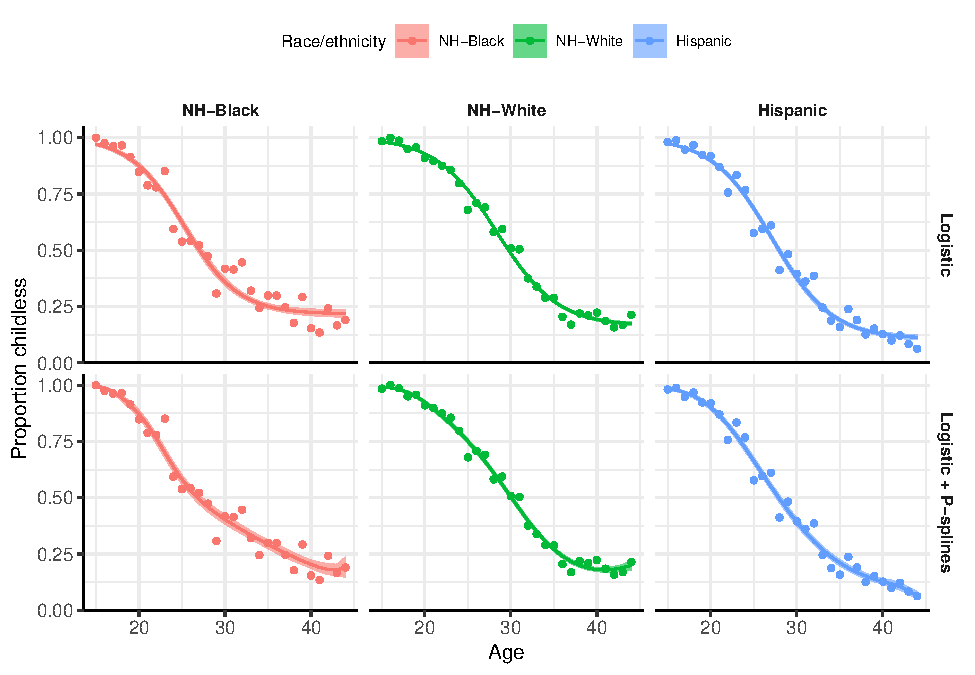
\includegraphics{childlessness_paa_ext_abstract_files/figure-latex/race-fit-1} \caption{Proportion of women childless by race/ethnicity with and without deviations from a logistic function during the year 2020}\label{fig:race-fit}
\end{figure}

Figure \ref{fig:pars-race} shows the median posterior estimates of the three logistic parameters over the period 1990-2020. The right-panel reflecting the function's midpoint (\(\delta\)) shows an upward trend, especially visible for Hispanic and non-Hispanic Black populations. This can be interpreted as a postponement of childbearing as it translates into the logistic function being shifted to the right (i.e to older ages). In line with the previous observation, the steepness of the curve (\(\gamma\)) shows a slight downward trend for all races/ethnicities. This illustrates that childbearing are spread over a wider age range. The middle panel showing the supremum of the function (\(\zeta\)) does not reflect any particular pattern.

\begin{figure}[H]
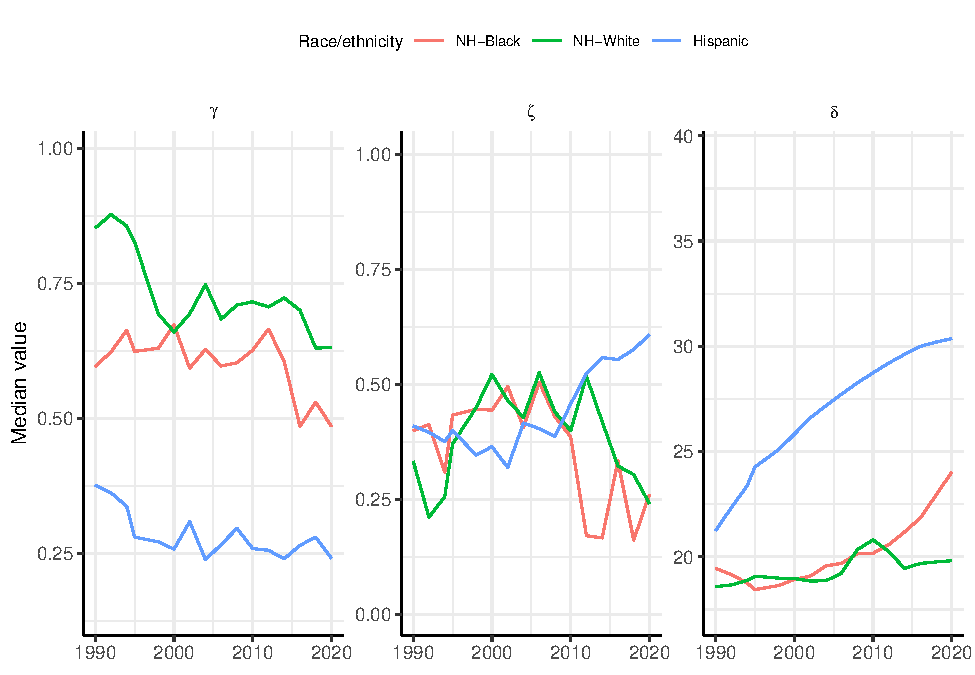
\includegraphics{childlessness_paa_ext_abstract_files/figure-latex/pars-race-1} \caption{Median posterior estimates of the logistic parameters over the period 1990-2020}\label{fig:pars-race}
\end{figure}

\hypertarget{next-steps-extensions}{%
\section{Next Steps \& Extensions}\label{next-steps-extensions}}

In this abstract we proposed a modeling framework to estimate age-specific proportions of women being childless. We propose a semi-parametric model consisting of a logistic function plus some deviations modeled with P-splines. Preliminary results shown for childlessness by racial/ethnic groups are promising.

Future work will model childlessness by U.S. state and racial/ethnic group. This modeling framework can also be used to project childlessness proportions of different subpopulation groups in the future. Finally, this modeling framework could be expanded to estimate simultaneously different parities by using a Multinomial data model with a series of constrained (semi)-parametric functions.

\newpage

\hypertarget{references}{%
\section*{References}\label{references}}
\addcontentsline{toc}{section}{References}

\hypertarget{refs}{}
\begin{CSLReferences}{1}{0}
\leavevmode\vadjust pre{\hypertarget{ref-de2012smoothing}{}}%
De Beer, J. (2012). Smoothing and projecting age-specific probabilities of death by TOPALS. \emph{Demographic Research} 27:543--592.

\leavevmode\vadjust pre{\hypertarget{ref-dye2010fertility}{}}%
Dye, J. (2010). Fertility of american women: 2008. Current population reports, P20--563. \emph{Washington, DC: US Census Bureau}.

\leavevmode\vadjust pre{\hypertarget{ref-dykstra2007pathways}{}}%
Dykstra, P.A. and Wagner, M. (2007). Pathways to childlessness and late-life outcomes. \emph{Journal of Family Issues} 28(11):1487--1517.

\leavevmode\vadjust pre{\hypertarget{ref-dyrting2020smoothing}{}}%
Dyrting, S. (2020). Smoothing migration intensities with p-TOPALS. \emph{Demographic Research} 43:1607--1650.

\leavevmode\vadjust pre{\hypertarget{ref-eilers1996flexible}{}}%
Eilers, P.H. and Marx, B.D. (1996). Flexible smoothing with b-splines and penalties. \emph{Statistical science} 11(2):89--121.

\leavevmode\vadjust pre{\hypertarget{ref-gemmill2019some}{}}%
Gemmill, A. (2019). From some to none? Fertility expectation dynamics of permanently childless women. \emph{Demography} 56(1):129--149.

\leavevmode\vadjust pre{\hypertarget{ref-gonzaga2016estimating}{}}%
Gonzaga, M.R. and Schmertmann, C.P. (2016). Estimating age-and sex-specific mortality rates for small areas with TOPALS regression: An application to brazil in 2010. \emph{Revista Brasileira de Estudos de Popula{ç}{ã}o} 33:629--652.

\leavevmode\vadjust pre{\hypertarget{ref-gray2013childbearing}{}}%
Gray, E., Evans, A., and Reimondos, A. (2013). Childbearing desires of childless men and women: When are goals adjusted? \emph{Advances in life course research} 18(2):141--149.

\leavevmode\vadjust pre{\hypertarget{ref-kendig2007health}{}}%
Kendig, H., Dykstra, P.A., Gaalen, R.I. van, and Melkas, T. (2007). Health of aging parents and childless individuals. \emph{Journal of Family Issues} 28(11):1457--1486.

\leavevmode\vadjust pre{\hypertarget{ref-kirmeyer2011childbearing}{}}%
Kirmeyer, S. and Hamilton, B.E. (2011). \emph{Childbearing Differences Among Three Generations of US Women}. Citeseer.

\leavevmode\vadjust pre{\hypertarget{ref-livingston2015childlessness}{}}%
Livingston, G. (2015). Childlessness falls, family size grows among highly educated women.

\leavevmode\vadjust pre{\hypertarget{ref-lundquist2009race}{}}%
Lundquist, J.H., Budig, M.J., and Curtis, A. (2009). Race and childlessness in america, 1988--2002. \emph{Journal of Marriage and Family} 71(3):741--755.

\leavevmode\vadjust pre{\hypertarget{ref-mynarska2015diverse}{}}%
Mynarska, M., Matysiak, A., Rybińska, A., Tocchioni, V., and Vignoli, D. (2015). Diverse paths into childlessness over the life course. \emph{Advances in life course research} 25:35--48.

\leavevmode\vadjust pre{\hypertarget{ref-nisen2014age}{}}%
Nisén, J., Martikainen, P., Silventoinen, K., and Myrskylä, M. (2014). Age-specific fertility by educational level in the finnish male cohort born 1940--1950. \emph{Demographic research} 31:119--136.

\end{CSLReferences}


\end{document}
